\documentclass[10pt,journal,letterpaper]{IEEEtran}
\usepackage[margin=1in]{geometry}
\usepackage{amsmath,amssymb,graphicx,booktabs,array,cite,url}
\renewcommand{\ttdefault}{cmtt}
\usepackage[hidelinks]{hyperref}
\hypersetup{pdftitle={Structured Channel Estimation for Rydberg Arrays With Learned Filtering and Observable Recovery Checks},pdfauthor={Abdullah Haatim}}
\graphicspath{{figures/}}
\interdisplaylinepenalty=2500
\newcommand{\CN}{\mathcal{CN}}
\newcommand{\HH}{\mathcal{H}}
\DeclareMathOperator{\diag}{diag}
\DeclareMathOperator{\tr}{tr}
\DeclareMathOperator{\sigmoid}{sigmoid}
\DeclareMathOperator{\softplus}{softplus}
\DeclareMathOperator{\median}{median}
\hyphenation{Ryd-berg mea-sure-ments}
\begin{document}
\title{Structured Channel Estimation for Rydberg Arrays With Learned Filtering and Observable Recovery Checks}
\author{Abdullah~Haatim\thanks{A. Haatim is with the Department of Electrical and Electronics Engineering, Birla Institute of Technology and Science, Pilani, India (e-mail: f20220519@pilani.bits-pilani.ac.in).}}
\maketitle
\begin{abstract}
Referenced magnitude measurements permit channel estimation in Rydberg array models without direct complex baseband observations. Hankel filtering can suppress noise but also erase useful spatial components or preserve an unfavorable initialization. We combine classical structural analysis with a compact self-supervised controller and an observable recovery check. The controller learns smooth Hankel filtering inside exact Rician expectation--maximization updates using withheld observations, without true-channel targets. A frozen hybrid uses an adaptive start at ordinary signal-to-noise ratios, a trained fixed schedule at higher ratios, and selected classical refinement. An antenna-residual check can invoke intensity regression and short EM refinement, accepting the alternative only when fitting likelihood improves. Independent development confirmation precedes a fresh paired comparison over 153 conditions and 1,152 physical channel realizations. The check improves equal-cell mean NMSE by 0.507 dB over its prior hybrid and 3.232 dB in the targeted weak-reference region, while observed BER is unchanged. The slower timing window gives 7.254 ms p90 against a 10.74 ms target. Compact sparse estimation retains better aggregate BER and pooled linear NMSE. The results support a conditional accuracy--cost trade-off under calibrated references, known noise variance and Gaussian fitting pilots.
\end{abstract}
\begin{IEEEkeywords}
Channel estimation, Hankel matrices, phase retrieval, Rydberg receivers, self-supervised learning.
\end{IEEEkeywords}

\section{Introduction}
\IEEEPARstart{R}{ydberg} atomic receivers sense radio-frequency electric fields through highly excited atoms. Their sensitivity and broad operating range motivate research on wireless communication and sensing, including future networks~\cite{gong2025mag}. Array models extend this setting to multiple users~\cite{cui2025}. In the magnitude-only receiver considered here, a known reference combines with the incoming field before amplitude measurement. The receiver does not directly observe complex baseband samples. Recovering the complex channel is therefore a nonlinear inverse problem, even when the pilots and reference are known.

A small number of propagation paths also gives the channel structure across the array. A Hankel matrix built from a uniform linear array channel has low rank. Filtering this matrix can suppress noise, but hard truncation can erase weak paths. The appropriate amount of filtering depends on the measurements and on channel complexity. Searching for a rank separately for every received block can be expensive. This motivates a practical question: can a small learned rule reuse offline training to provide useful structural correction at lower processing cost, and when does a well-tuned classical method remain better?

We develop one receiver framework with three contributions. First, a compact controller adapts smooth spatial Hankel filtering within exact referenced-Rician EM updates, with training based on withheld observations rather than true-channel targets. Classical array-size and effective-rank studies explain the structural benefit and its bias; individual-update bounds state precisely what is, and is not, guaranteed. Second, a frozen hybrid combines adaptive and globally trained schedules with short classical refinement and an observable residual/likelihood recovery wrapper. Its alternative algebraic start provides a distinct recovery route when estimates derived from the common spectral start fit poorly. Third, independent confirmation of the added recovery rule and fresh paired NMSE, BER and serial-time comparisons quantify this combination under a fixed percentile budget, including unfavorable cells and metric-dependent rankings.

These are contributions of a particular design, analysis and controlled evaluation. Exact EM, Hankel low rank, learned unfolding, withheld-data training and affine-intensity regression are established ideas. The algebraic replacement is classical; its gains cannot be credited uniquely to learning. Our evidence distinguishes a reusable adaptive component from the additional value of the complete hybrid, and does not establish uniform superiority over classical estimation.

\subsection{Relation to Existing Work}
Cui et al.\ developed EM-based Gerchberg--Saxton (EM-GS) for atomic-MIMO detection~\cite{cui2025}; we apply it to known-pilot channel estimation. Unlike strong-reference linearization~\cite{xu2025}, we retain exact magnitudes. URformer already unfolds Rydberg phase retrieval~\cite{xiao2026}, replacing the Bessel filter with a learned module and training against true-channel NMSE. Our design retains the exact Bessel update and learns spatial filtering from withheld observations. We do not reproduce URformer's published performance or claim a matched accuracy advantage over it. Quantum-MUSIC and its robust variant address direction finding and outliers~\cite{kim2025quantummusic,banerjee2026robust}, not the estimation trade-off studied here.

Classical structure processing includes Cadzow's alternating projections~\cite{cadzow1988}, Hankel recovery~\cite{chen2014emac}, low-rank Hankel denoising (LRHD)~\cite{yin2021}, and structured alternating least squares~\cite{zachariah2012}. OptShrink chooses data-driven singular-value weights~\cite{nadakuditi2014}. Variational Bayesian low-rank phase retrieval~\cite{liu2018lrpr} and Vandermonde factorization~\cite{ying2018hvaf} offer other priors. Their original observations and guarantees differ from referenced Rician recovery. Our in-loop OptShrink adaptation is a strong control, not a reproduction of full LRHD or these other methods. Their guarantees are not transferred to the dependent errors produced by nonlinear reconstruction and Hankel lifting.

Compact learned estimators also have clear precedents. C-TISTA uses four scalars per stage for complex inverse problems~\cite{takabe2020ctista}. ALISTA retains analytic weights and learns steps and thresholds~\cite{liu2019alista}; OAMP-Net2 uses four scalars per stage for MIMO detection~\cite{he2020oamp}. NA-ALISTA uses recurrence and observed residual summaries to control sparse recovery~\cite{behrens2021naalista}. Compactness and input-dependent control are not new by themselves. Learned Hankel reconstruction~\cite{huang2021}, withheld-measurement self-supervision~\cite{yaman2020,luo2023}, Rician-likelihood learning~\cite{parker2023}, and self-supervised Rydberg-signal denoising~\cite{liu2026} also precede this work. Affine phase retrieval~\cite{gao2018} and intensity lifting~\cite{candes2013phaselift,li2020affinelift} also precede our algebraic alternative. Its nuisance-parameter least-squares implementation and validity analysis are specialized to the repeated-reference model; they are not a new lifting principle. Our specific learned design adjusts smooth spatial Hankel filtering inside exact referenced-magnitude EM. The matched recurrent control tests one adaptation of that broader idea, not superiority over published NA-ALISTA.

\section{System Model and Available Information}
\begin{figure*}[!t]
\centering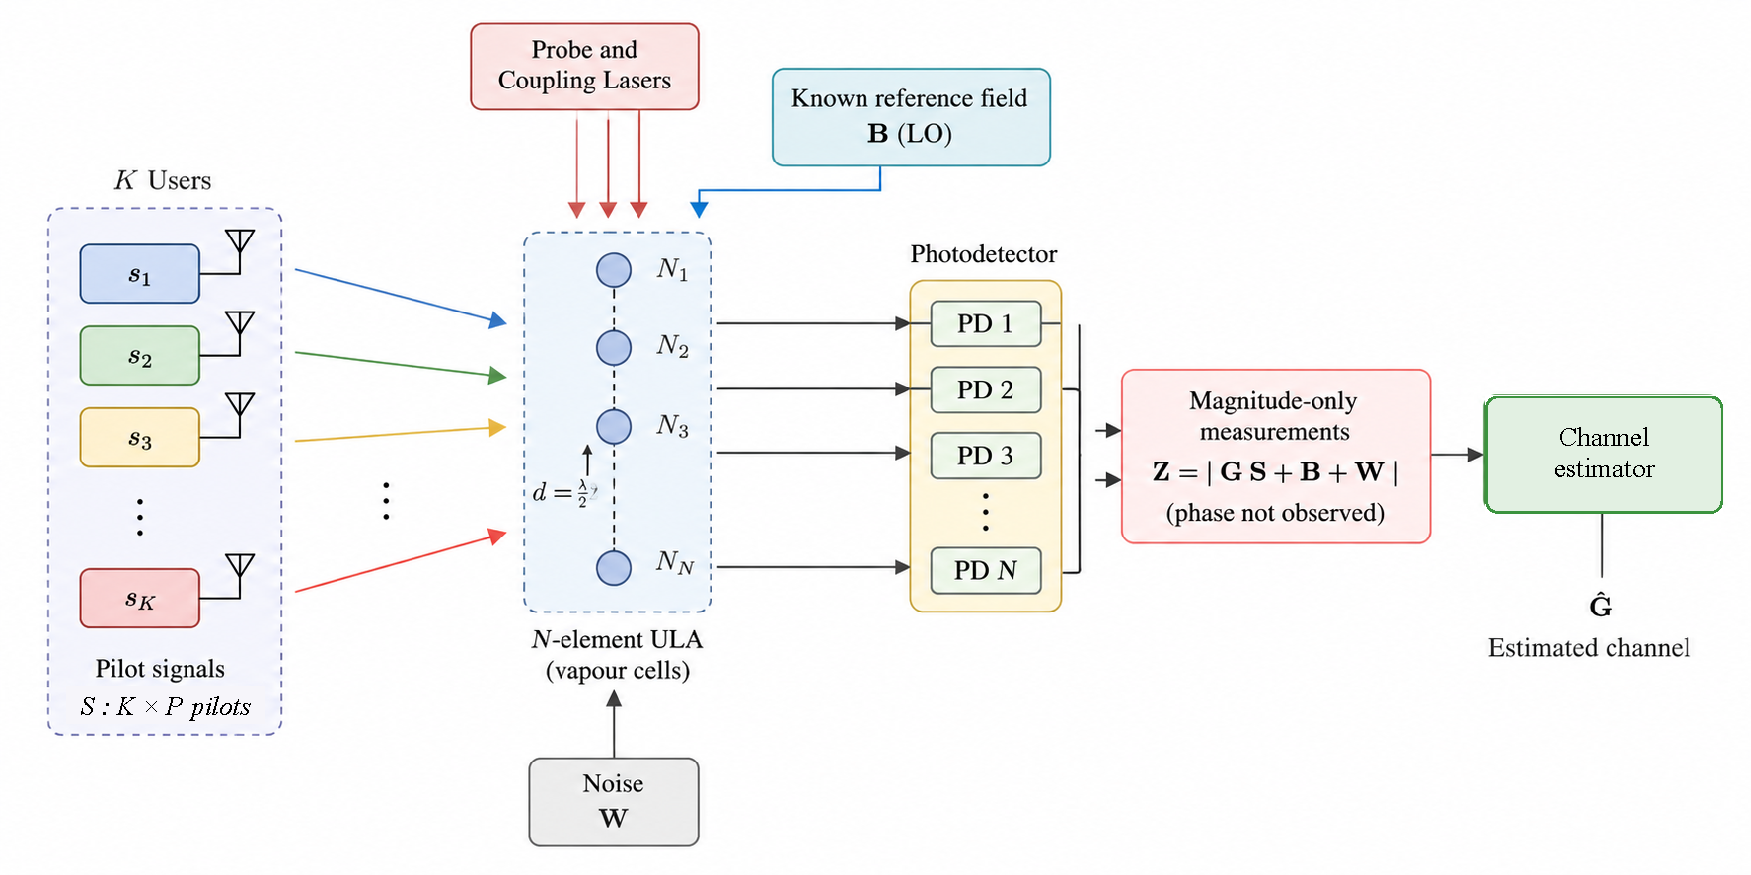
\includegraphics[width=\textwidth]{system_model.pdf}
\caption{Uplink receiver model. $K$ users send pilots to $N$ vapour-cell elements in a half-wavelength uniform linear array. A known RF reference combines with the received field. The optical readout supplies magnitude-only measurements to a channel estimator, covering both classical and learned methods. Lasers and photodetectors are schematic; atomic dynamics and optical readout are not simulated.}
\label{fig:system}
\end{figure*}
Figure~\ref{fig:system} shows the receiver. An $N$-element array receives $P$ pilots from $K$ users:
\begin{equation}
 Z=|GS+B+W|,\qquad W_{np}\sim\CN(0,v).
 \label{eq:model}
\end{equation}
Here $G\in\mathbb C^{N\times K}$ is the unknown channel, $S\in\mathbb C^{K\times P}$ contains known pilots, and $B$ is the known reference field. Magnitude acts entrywise. Noise samples are independent, with variance $v/2$ in each real component. Receiver conversion gain is absorbed into the scaling. This effective model does not simulate atomic dynamics, optical readout or hardware drift.

For a half-wavelength uniform linear array, user $k$ has channel
\begin{equation}
 g_{nk}=\sum_{\ell=1}^{L_k}\alpha_{\ell k}e^{-j\pi n\sin\theta_{\ell k}},
 \quad n=0,\ldots,N-1.
 \label{eq:channel}
\end{equation}
We draw $\alpha_{\ell k}\sim\CN(0,1/L_k)$ and independent angles uniformly on $(-\pi/2,\pi/2)$. Pilots follow $\CN(0,1)$. The reference is broadside with constant waveform and zero phase:
\begin{equation}
 B_{np}=10^{\mathrm{RSR}/20},\qquad v=K10^{-\mathrm{SNR}/10}.
\end{equation}
SNR is relative to aggregate user power; reference-to-signal ratio (RSR) is relative to one user's power. At $K=3$, RSR 12~dB is 7.23~dB relative to total signal power. Each user's expected channel power is one; individual realizations are not normalized to identical energy. Main comparisons supply the correct reference and noise variance to every estimator.

\subsection{Likelihood, Ambiguity and Local Recovery}
For $a=|\mu|$, a magnitude observation has Rician density
\begin{equation}
 p(z\mid a,v)=\frac{2z}{v}e^{-(z^2+a^2)/v}I_0(2za/v),\quad z\ge0.
\end{equation}
For fixed $v$, its negative log-likelihood, up to observation-only terms, is
\begin{equation}
 \ell(z,\mu,v)=\frac{(z-|\mu|)^2}{v}-\log I_{0e}(2z|\mu|/v),
 \label{eq:loss}
\end{equation}
where $I_{0e}(x)=e^{-x}I_0(x)$ for $x\ge0$. Scaled Bessel functions avoid overflow. If variance is estimated, the omitted $\log v$ term must be restored.

For one array row, write $\mu_p=g^Ts_p+b_p$ and use real coordinates $x=[\operatorname{Re}g^T,\operatorname{Im}g^T]^T$. At nonzero $\mu_p$, the noiseless magnitude Jacobian has row
\begin{equation}
 A_p=[\operatorname{Re}c_p^T,-\operatorname{Im}c_p^T],\qquad
 c_p=\mu_p^*s_p/|\mu_p|.
 \label{eq:jacobian}
\end{equation}
If $A$ has rank $2K$, an invertible square sub-Jacobian gives local recovery by the inverse function theorem. Thus $P\ge2K$ is necessary for this regular full-rank condition, but not sufficient. A small minimum singular value also makes recovery sensitive to noise. This is a local statement for an unrestricted row, not a global or sparse-channel recovery theorem~\cite{gao2018}.

With $B=0$, multiplying $g$ by a common phase leaves its magnitudes unchanged. A nonzero reference can break this ambiguity, but not for every design. If $b_p=c^Ts_p$, rotating $g+c$ still preserves the observations. An unknown common reference phase also allows simultaneous rotation of channel and reference. Absolute phase cannot then be recovered without another phase anchor. Known reference calibration is a substantive assumption, not just a choice of units.

\subsection{Information References}
For independent measurements, the real Fisher information is
\begin{align}
 J&=A^T\diag(w_p)A,\nonumber\\
 w_p&=\mathbb E\!\left[\left(-\frac{2a_p}{v}+\frac{2Z_p}{v}
 \frac{I_1(2Z_pa_p/v)}{I_0(2Z_pa_p/v)}\right)^2\right].
\end{align}
One magnitude contributes at most one information direction. The full channel information combines array rows in the same real-coordinate ordering. Where the required matrices are nonsingular, the unrestricted reference is $J^{-1}$. The geometric constrained Cram\'er--Rao bound (CCRB) is~\cite{stoica1998}
\begin{equation}
 C_{\rm geom}=U(U^TJU)^{-1}U^T,
 \label{eq:ccrb}
\end{equation}
where $U$ spans the real tangent space at the true path configuration. With $\omega=\pi\sin\theta$, its complex derivative columns are $e^{-jn\omega}$, $je^{-jn\omega}$ and $-jn\alpha e^{-jn\omega}$. Real and imaginary stacking gives the tangent basis. True path count is used only for this ideal diagnostic.

We normalize summed traces by summed channel energy. The gap between these references describes the local value of geometric information under unbiasedness assumptions. It is not guaranteed attainable improvement. Our filtered estimators can be biased, so these curves are not absolute lower limits on their measured error.

\section{Classical Structural Estimation}
\subsection{Exact Rician Measurement Update}
Let $M=GS+B$ and $\kappa=2Z|M|/v$. Conditional averaging of the unobserved complex field gives
\begin{align}
 Q&=Z\odot\frac{I_1(\kappa)}{I_0(\kappa)}\odot\frac{M}{|M|},\nonumber\\
 G_{\rm EM}&=(Q-B)S^H(SS^H)^{-1}.
 \label{eq:em}
\end{align}
Ratios act entrywise; the first line has continuous limit zero at $M=0$. A linear solve evaluates the second line, requiring a full-row-rank fitting pilot matrix. For $\mathcal L(G)=\sum_{np}\ell(Z_{np},M_{np},v)$,
\begin{align}
 D&=\frac{\partial\mathcal L}{\partial G^*}=\frac{(M-Q)S^H}{v},\nonumber\\
 G_{\rm EM}&=G-vD(SS^H)^{-1}.
\end{align}
EM is therefore an exact preconditioned gradient update for this likelihood. The packed real gradient is $2D$; this factor matters when comparing gradient-based and EM-based stages.

The trained and direct-EM starts use the following spectral initialization; the alternative intensity-regression start in Section~\ref{sec:receiver} deliberately differs. For row $n$, form $C_n$ with rows $[s_p^T,b_{np}]$ and take the leading eigenvector $u_n$ of $C_n^H\diag(z_n)C_n$. Set
\begin{equation}
 c_n=\frac{\sum_p z_{np}|(C_nu_n)_p|}{\sum_p|(C_nu_n)_p|^2}.
\end{equation}
The first $K$ entries of $c_nu_ne^{-j\arg(u_{n,K+1})}$ initialize the channel row. When observations are withheld, only the fitting subset enters initialization. Otherwise the estimator would contain information from its validation observations.

\subsection{Hankel Lifting and Rank Selection}
Let $q=\lceil N/2\rceil$, $m=N-q+1$, and
\begin{equation}
 [\HH(g)]_{ij}=g_{i+j},\quad 0\le i<m,\quad0\le j<q.
\end{equation}
A channel with $L$ distinct spatial frequencies has Hankel rank at most $\min(L,m,q)$. The inverse map $\HH^\dagger$ averages antidiagonals and satisfies $\HH^\dagger\HH(g)=g$. A hard-rank sweep retains the largest $r$ singular components and then averages antidiagonals. Repeating these operations is a Cadzow procedure; finitely many sweeps do not give an exact projection onto the intersection of Hankel and rank constraints.

Our Hankel-structured GS (HS-GS) baseline applies these sweeps after each EM update. It fits candidate shared user ranks $r=1,\ldots,q$ on the first 70\% of pilots and selects the smallest held-out squared amplitude residual on the remainder. It then restarts on all pilots. Unless specified otherwise, candidate/final budgets are 25/100 EM updates and each update uses four sweeps. Rank $q$ explicitly bypasses filtering and recovers the paired EM-GS output. This option does not guarantee that validation chooses the bypass whenever filtering is harmful. We call amplitude-loss selection HS-amplitude and Rician-loss selection HS-Rician. Shared rank is a computational choice, not an assumption of equal user path counts.

\subsection{Smooth Filtering and OptShrink Controls}
The smooth operation replaces each singular value by
\begin{equation}
 \widehat\sigma_i=\frac{\sigma_i^3}{\sigma_i^2+\tau^2}.
 \label{eq:shrink}
\end{equation}
A classical control selects $\tau$ as a multiple of the current RMS singular value, using held-out amplitude error. Multipliers are $\{0,0.05,0.1,0.2,0.4,0.8,1.6\}$; zero bypasses filtering. Update and selection budgets match HS-amplitude. This empirical rule is not OptShrink and has no claimed statistical optimality.

OptShrink instead estimates retained weights from the discarded spectrum~\cite{nadakuditi2014}. For singular values $s_1\ge\cdots\ge s_q$ and candidate rank $r<q$, define
\begin{align}
 \phi_d(z)&=\frac{1}{d-r}\left[\sum_{j=r+1}^{q}\frac{z}{z^2-s_j^2}+\frac{d-q}{z}\right],\nonumber\\
 \mathcal D(z)&=\phi_m(z)\phi_q(z),\quad
 \widehat s_i=-2\mathcal D(s_i)/\mathcal D'(s_i),\ i\le r.
\end{align}
Other weights are zero. We rescale the spectrum, guard unresolved poles, average antidiagonals and mix the result with the measurement update. The adaptation is applied either after every update or once at the end.

In the historical OptShrink study, the broad offline search uses the original learned estimator's 2,048 validation observations and the same 21/9 masks. It covers both placements, ranks 1--15 plus no filtering, mixing factors $0.25,0.5,0.75,1$, and update budgets $5,10,20,50,100$: 610 combinations. Rician validation loss is averaged equally over six path regimes. Settings are frozen for each of 21 noise/reference pairs before testing. Path labels balance offline selection; they are not inference inputs. Off-grid stress tests use the nearest lookup without retuning.

A stronger in-loop control selects rank for each received block. It keeps the lookup's mixing and iteration budget, fits ranks 1--15 plus bypass to 21 pilots, scores nine held-out pilots with Rician loss, and restarts on all 30. All search and refitting time counts. This is not an unrestricted search over user-specific ranks, mixing factors and stopping times. It uses no extra pilot observations, but pays computation to use the current block rather than only offline averages.

\section{Compact Self-Supervised Estimator}
\subsection{Measurement and Structural Stages}
Each learned start uses ten stages. At stage $t$, it relaxes the exact EM update:
\begin{equation}
 G_{\rm dc}=G+\gamma_t(G_{\rm EM}-G),\qquad
 \gamma_t=2\sigmoid(a_t).
\end{equation}
The ten learned $a_t$ start at $\gamma_t=1$. For user $k$, write $H_k=\HH(g_{{\rm dc},k})$, $s_H=\|H_k\|_F/\sqrt q$, and $p_i=\sigma_i/\sum_j\sigma_j$. A shared 8--16--2 network with SiLU activation receives
\begin{align}
 f_1&=\exp(-\textstyle\sum_i p_i\log p_i)/q,\quad f_2=p_1,\nonumber\\
 f_3&=\textstyle\sum_{i=q-\lceil q/2\rceil+1}^q p_i,\nonumber\\
 f_4&=\log\!\left(1+\operatorname{mean}[(Z-|G_{\rm dc}S+B|)^2]/v\right),\nonumber\\
 f_{5,k}&=\log\!\left(1+v\tr[(SS^H)^{-1}]/(K\widehat p_k)\right),
 \label{eq:features}
\end{align}
and $P/(2K)$, $\log q$, $(t+1)/10$. Here $\widehat p_k=\|g_{{\rm dc},k}\|_2^2/N$, $t=0,\ldots,9$, and the residual mean uses all fitting observations. These inputs describe the current spectrum, residual, noise, pilot support, size and stage. They contain no true channel, true rank or generator label.

Outputs $(u,w)$ set $\tau=s_H[0.001+\softplus(u)]$ and $\beta=\sigmoid(w)$. The smooth filter and channel update are
\begin{align}
 F_\tau(H)&=H-\tau^2H(H^HH+\tau^2I)^{-1},\label{eq:solve}\\
 g_k^{t+1}&=g_{{\rm dc},k}+\beta_{t,k}
 [\HH^\dagger F_{\tau_{t,k}}(H_k)-g_{{\rm dc},k}].
\end{align}
The solve implements~\eqref{eq:shrink} after normalization by $s_H$. Gradients pass through it without an identity-backward approximation. Spectral features still require singular values. Threshold and mixing start near $0.1s_H$ and 0.1. The network has 178 parameters; ten EM steps bring the total to 188.

For reproducibility, channel power and singular-value sum are floored at $10^{-12}$, and squared Hankel RMS scale at $10^{-24}$. Pilot-Gram systems use direct solves without an added ridge. PyTorch implementations use scaled Bessel functions and a series for $\kappa^2<10^{-4}$. OptShrink zeros weights at relative squared spectral gaps at most $10^{-13}$. These are fixed numerical rules, not tuned extra physical assumptions. Positive threshold makes the reconstruction solve smooth, although ordered spectral features need not be differentiable at every tie.

Threshold and gate can compensate for each other. The gate is often near one in the fitted models; most adaptation changes filtering strength rather than providing an on/off decision. Neither output is an estimated physical rank. We measure actual correction by $\|g_k^{t+1}-g_{{\rm dc},k}\|_2/(\|g_{{\rm dc},k}\|_2+\epsilon)$ rather than interpreting the gate alone as reliable abstention.

\subsection{Learning Without True-Channel Targets}
For the final learned components, each offline block contains 39 simulated observations. A changing random split assigns 30 context columns $A$ and nine disjoint withheld columns $V$ with independent measurement noise. The pilot matrix is screened jointly before splitting. Only context data enter initialization, features and updates. Training minimizes
\begin{equation}
 \mathcal L_{\rm hold}=\frac{1}{N|V|}\sum_{n,p\in V}
 \ell\big(Z_{np},[\widehat G_A S_V+B_V]_{np},v\big).
\end{equation}
Gradients pass through the ten stages, so a threshold or mixing change is rewarded when it predicts the withheld magnitudes more accurately. The loss needs no true channel. Independent validation blocks use fixed masks; the mean held-out loss over 126 reference/SNR/path strata selects the checkpoint, including the untrained candidate. All 30 available pilots enter the frozen estimator at deployment. There is no online fitting of network weights.

Both adaptive and global models use 16,384 training blocks, 2,048 validation blocks, Adam at learning rate $10^{-3}$, batch size 32 and 20 epochs. Half the blocks have independent 3--7 paths per user; the rest allocate shared path counts $2,4,8,12,16$. Seven SNRs from $-10$ to 20~dB and references 5, 12 and 20~dB define the validation strata. The two families share observation banks, masks, batch orders and initial update/filter outputs. Seeds 9101--9103 provide three paired fits on one shared training population. Training is single precision and final inference is double precision. A common finite budget is not proof of convergence or uncertainty across new training populations.

This matched 30-context protocol differs from both the original 21/9 split within 30 observations and the historical all-pilot re-corruption experiment. The latter changed training noise and loss as well as pilot use. Their evidence is retained separately in the supplement. The final neural components still use self-supervised channel learning; subsequent policy development also uses known-symbol communication probes and is not entirely unlabeled.

\subsection{Compact Controls and Parameter Accounting}
A step-only control learns ten relaxation parameters. A global schedule learns one relaxation, relative threshold and mixing factor per stage, giving 30 parameters. Its absolute threshold remains scaled by the observed Hankel RMS, although the stage constants are fixed after training. The adaptive design has 188 parameters. Historical matched comparisons also include a 148-parameter recurrent controller inspired by NA-ALISTA, using residual and update-displacement inputs with a four-unit LSTM. This is a model-specific adaptation rather than a reproduction of published NA-ALISTA. Features, recurrence and controlled quantities differ; its result cannot isolate a single architectural cause. The final hybrid stores one adaptive and one global fit, and its additional classical recovery branch has no learned weights.

\subsection{Properties of Individual Updates}
Define $F_0(H)=H$ by continuity. For fixed $\tau>0$, each multiplier in~\eqref{eq:shrink} lies in $[0,1]$. Therefore
\begin{equation}
 \|F_\tau(H)\|_F\le\|H\|_F,\qquad
 \|F_\tau(H)-H\|_F\le\sqrt q\,\tau/2.
 \label{eq:bound}
\end{equation}
The second result follows by maximizing $\sigma\tau^2/(\sigma^2+\tau^2)$, whose maximum is $\tau/2$. Let $D_H$ contain antidiagonal multiplicities, so $\|g\|_{D_H}=\|\HH(g)\|_F$. Antidiagonal averaging is the lifted-space orthogonal projection onto Hankel matrices. The gated step thus does not increase this weighted norm and has weighted correction at most $\beta\sqrt q\tau/2$. This bounds the step's output, not its error relative to the true channel or contraction between two inputs.

The EM surrogate is $\|Q-B-GS\|_F^2/v$. Its normal equations show that relaxation reduces this surrogate by
\begin{equation}
 \gamma_t(2-\gamma_t)\|(G-G_{\rm EM})S\|_F^2/v\ge0
\end{equation}
for $0\le\gamma_t\le2$. Subsequent filtering need not decrease the surrogate or likelihood. No convergence, fixed-point stability or low-noise consistency theorem follows for the full estimator. In particular, the learned threshold need not vanish with noise. The acceptance wrapper in Section~\ref{sec:receiver} guarantees only fitting-loss nonincrease relative to its incumbent, not smaller channel error. Cubic shrinkage remains a design choice, not a statistically optimal filter for the induced Hankel errors.

\section{A Receiver With Observable Recovery Checks}
\label{sec:receiver}
The adaptive controller is useful at ordinary SNR but is not an adequate complete receiver over the extended operating range. We therefore freeze a hybrid that combines the two matched-context trained starts with classical refinement and an alternative initialization. All routing uses measurements, the supplied reference and variance, and stored constants. Neither the channel, its path count, its error nor test BER is an inference input.

\subsection{Regime Routing and Noise-Scaled Final Filtering}
Define nominal proxies $s=10\log_{10}(K/v)$ and $r=10\log_{10}\operatorname{mean}|B|^2$. They equal the generator's SNR and RSR under the stated normalization; they are not estimates of instantaneous channel power. For $s\le20$~dB, the receiver returns the matched-context adaptive output without extra EM or a final filter. It also uses the adaptive start through 30~dB; above 30~dB it uses the global schedule. The global schedule is trained, although its stage parameters are fixed after training. Only one start is evaluated for each block. A paired deployed fit stores $188+30=218$ neural parameters, in addition to the discrete policy and numerical constants.

Above 20~dB, a frozen reference/SNR table selects $T\in\{0,10,20,40\}$ exact EM continuation updates and a final multiplier $c\in\{0,2,4\}$. Continuation starts from the trained estimate, without spectral reinitialization. Let $V_S=(SS^H)^{-1}$. The final userwise filter uses
\begin{equation}
 \tau_k=c\sqrt{2v\operatorname{Re}[V_S]_{kk}\max(m,q)},\qquad \beta=1,
 \label{eq:finaltau}
\end{equation}
with $c=0$ denoting a bypass. This is a heuristic noise scale, not the covariance of a nonlinear channel estimate. Reference and SNR lookup use the nearest declared grid values, choosing the lower bin at an exact tie. A mismatch between the continuously selected model family and the table's family gives zero extra EM. The supplement gives every table entry and numerical boundary tolerance.

The strong-reference final filter remains active across 40~dB, avoiding the earlier imposed filter-removal jump. This does not make the entire receiver continuous: the model crossover and other table boundaries remain. Let $G_0$ denote the complete output of this frozen prior hybrid, including any continuation and final filtering.

\subsection{A Residual Check Without Channel Truth}
The new check is restricted to the nearest-reference 5~dB bin and continuous $s>30$~dB. Compute
\begin{equation}
 R_n=\frac{2}{Pv}\sum_p\bigl(Z_{np}-|[G_0S+B]_{np}|\bigr)^2.
 \label{eq:gate}
\end{equation}
The selected rule triggers when $\max_nR_n>2$. It examines the largest antenna residual because a poor row estimate can be diluted in an array average. The factor two reflects the high-SNR amplitude-noise scale; the maximum of fitted residuals is not a calibrated statistical test or a failure probability. When the condition is ineligible or the threshold is not crossed, the output is exactly $G_0$.

\subsection{An Algebraic Alternative to the Shared Spectral Start}
All trained and direct-EM starts in this comparison share a spectral initialization and can inherit its unfavorable solutions. For a triggered case, exploit the repeated nonzero reference $B_{np}=b_n$. Set $c_n=g_n/b_n$ and
\begin{equation}
 y_{np}=\frac{Z_{np}^2-v}{|b_n|^2}-1.
\end{equation}
Since $\mathbb E|\mu+W|^2=|\mu|^2+v$,
\begin{equation}
 \mathbb E[y_{np}\mid G,S,B]
 =2\operatorname{Re}(c_n^Ts_p)+|c_n^Ts_p|^2.
 \label{eq:intensity}
\end{equation}
For $K=3$, construct a real $P\times15$ design $D$ containing six linear columns $2\operatorname{Re}s_i,-2\operatorname{Im}s_i$, three diagonal columns $|s_i|^2$, and six off-diagonal columns
\begin{equation}
 2\operatorname{Re}(s_i s_j^*),\quad
 -2\operatorname{Im}(s_i s_j^*),\qquad i<j.
\end{equation}
The nine quadratic coefficients are unrestricted Hermitian nuisance parameters. One SVD least-squares solve $D^\dagger Y$ shares the $N$ antenna right-hand sides. The first six coefficients recover $\operatorname{Re}c_n,\operatorname{Im}c_n$, after which $g_n=b_nc_n$. This is an affine-intensity regression construction related to established lifting methods~\cite{gao2018,candes2013phaselift,li2020affinelift}; we do not claim that reference-assisted linearization or algebraic phase retrieval is new.

\textit{Full-rank property.} If $v=0$, the reference repeats and is nonzero, and $D$ has column rank 15, the linear coefficients recover the true channel exactly. Indeed, expansion of $|c_n^Ts_p|^2$ gives an exact solution of $D\xi_n=y_n$; full column rank makes that solution unique. With the correct positive variance subtracted, the unfiltered least-squares estimate is conditionally unbiased by linearity of $D^\dagger$. Neither statement applies to the subsequent nonlinear refinement or selection as an unbiasedness guarantee.

The implementation requires rank 15, condition number at most $10^8$, and finite coefficients. It treats a failed solve as invalid. Constant-modulus fitting pilots make the three diagonal columns collinear and give rank at most 13. Thus the implemented fallback is rejected for QPSK fitting pilots; the current evidence concerns Gaussian fitting pilots. This restriction belongs to this redundant nuisance parameterization and rank rule, not to affine recovery in general.

\subsection{Refinement and Likelihood Acceptance}
A valid algebraic estimate receives 20 exact EM updates and the same final-filter rule as $G_0$. Denote it by $G_{\rm fb}$, and let $\overline{\mathcal L}$ be the average of~\eqref{eq:loss} over fitting observations. The receiver returns
\begin{equation}
 \widehat G=\begin{cases}
 G_{\rm fb},&\overline{\mathcal L}(G_{\rm fb})<
 \overline{\mathcal L}(G_0)-10^{-12},\\
 G_0,&\text{otherwise},
 \end{cases}
 \label{eq:accept}
\end{equation}
only after a trigger and a valid finite fallback. Invalid solves retain $G_0$. Acceptance replaces the complete channel estimate, not isolated rows. By construction, this wrapper never increases fitting loss relative to its computed incumbent. It does not guarantee lower channel error, BER or out-of-sample loss. This elementary comparison property is distinct from convergence of the complete receiver.

The receiver is evaluated in the following order: compute one trained start, perform its selected continuation and final filter, check eligibility and residuals, optionally compute and refine the algebraic alternative, then apply~\eqref{eq:accept}. All of this work is timed. There are no additional online pilots, true-channel decisions or online weight updates. A separate algebraic-plus-EM20 control measures the value of the classical alternative on its own; its invalid-solve branch uses spectral initialization plus 20 EM updates rather than retaining $G_0$.

\section{Experimental Design}
\label{sec:protocol}
\subsection{Historical Evidence and the Final Comparison}
We keep distinct studies separate. The classical array study uses $K=3$, $N=8,16,32$, $P=10,30$, RSR 12~dB, six SNRs from $-5$ to 20~dB and 400 paired worlds per cell. Unless fixed, user path counts are independently uniform on 3--7. It rejects circular spatial-frequency separation below $10^{-10}$, steering-matrix singular-value ratio below $10^{-8}$ and pilot singular-value ratio below $10^{-8}$. Effective-rank studies use $N=16,32,64$, $P=20$, RSR 10~dB and 300--400 worlds per cell with SNR uniform on $[-10,20]$~dB. The smooth/hard-filter comparison uses $N=32$, $P=30$, RSR 12~dB, $L=3,7,14$ and SNR 0 and 10~dB, with 400 worlds per cell. These screened classical samples and their information references are not pooled with the final receiver results.

The final comparison fixes $N=32$, $K=3$, $P=30$ and crosses three references $\{5,12,20\}$~dB, three path regimes (two paths per user, four paths per user, or independent 3--7 paths) and 17 SNRs:
\begin{equation*}
 \begin{gathered}
 \{0,5,10,15,20,22.5,25,27.5,30,32.5,\\
 35,37.5,40,42.5,45,50,60\}\ \mathrm{dB}.
 \end{gathered}
\end{equation*}
Each reference/path block contains 128 independently generated physical channel/pilot/noise anchors, with its own random-number domain. The same separation and singular-value screens apply to these channels and fitting pilots. Within a block, the same anchor is reused across SNR through noise scaling. There are 153 conditions, 19,584 condition cases and 1,152 physical anchors, not 19,584 independent channels. Methods and the three fixed trained fits share observations. Paths, fitting pilots and noise are independently redrawn across anchors. True channels score final errors but never enter receiver decisions.

\subsection{Development, Confirmation and Frozen Decisions}
The incumbent hybrid, learned weights and all baselines were fixed before this experiment. Its inherited selective-EM table came from an exploratory earlier proposal whose independent confirmation had failed. It remains an explicitly identified comparator; the new experiment does not retrospectively validate those earlier tail choices.

The new recovery rule was chosen from 12 predeclared combinations: antenna-mean or antenna-maximum residual, threshold $2,4,8$, and 10 or 20 fallback EM updates. A separate runtime calibration screened complete rules against 10~ms p90 both over the grid and in the weak-reference target region. All 12 passed. Forced-fallback timings were recorded separately. The incumbent was always admissible.

Development bank A and confirmation bank C each contain 256 independent anchors in each of the three path regimes at reference 5~dB, shared across the eight SNRs above 30~dB. Each development channel has 30 fitting pilots, nine independent held-out Gaussian pilots and 64 known joint-QPSK probe vectors with separate noise. The extra observations and symbol labels are available only offline. No true-channel targets or errors select the rule.

On A, a candidate must improve mean held-out Rician loss by more than $10^{-12}$ and not increase empirical probe bit errors in each path regime. Among eligible rules, the smallest equally weighted held-out loss wins. Fixed ties favor the incumbent, then fewer triggers, fewer EM steps, larger threshold and mean before maximum. Only that rule is tested on C: a positive one-sided 95\% bootstrap lower bound on pooled held-out-loss improvement and empirical BER nonincrease in every regime are required. No runner-up is tried if C fails. The selected maximum-residual/threshold-2/EM20 rule passes, with lower bound 0.1987. Both methods have zero observed C-probe errors; that is not formal BER noninferiority evidence. The policy and source/checkpoint hashes were frozen before generating the final test bank.

\subsection{Matched Baselines and Communication Evaluation}
The final table includes the prior hybrid, the earlier full repaired adaptive receiver, and adaptive, global and classical structured starts with the same 40 extra EM steps and final-filter table. Each start contains ten measurement/structure stages; zero \emph{extra} EM does not mean zero estimation iterations. The classical start uses fixed unit EM relaxation and an offline-selected smooth-filter threshold and mixing. Direct EM100 uses the shared spectral initializer. All receive the same 30 fitting pilots, reference and variance.

The compact sparse/EM baseline is an angle-domain Rician-likelihood adaptation with frozen reference/SNR selection. Of its 51 lookup bins, 34 use penalized sparse configurations with dictionary size 128 or 256 and 17 choose the zero-penalty direct-EM100 branch. It is not a sparse method at every operating point. The standalone algebraic-plus-EM20 method uses the initializer and invalid-solve rule in Section~\ref{sec:receiver}. Baseline calibration and all policy entries are retained in the supplement and evidence archive. OptShrink was omitted prospectively from this budget-focused final test because earlier measured p90 was approximately 79--81~ms. Historical OptShrink comparisons remain separate; none is presented as a fresh measurement in the final table. A matched implementation of published URformer is not included.

For BER, every estimate enters the same joint magnitude-domain detector:
\begin{equation}
 \widehat x=\arg\min_{x\in\mathcal Q^K}\sum_n
 \ell(z_n^{\rm d},\widehat g_n^Tx+b_n,v),
\end{equation}
where $\mathcal Q$ is unit-energy QPSK. Each channel transmits all 64 joint symbol vectors once, with independent data noise, giving 384 bits per condition case and 7,520,256 bits per trained fit over the grid. Data observations are identical across estimators and are unavailable to channel inference. Perfect-CSI detection is a diagnostic reference, not a deployable estimator. Data-noise draws remain coupled across SNR within each physical anchor.

\subsection{Metrics, Dependence and Runtime}
Let $e_{a,i}=\|\widehat G_{a,i}-G_i\|_F^2$ and $d_i=\|G_i\|_F^2$. Cell NMSE is
\begin{equation}
 E_a=10\log_{10}\frac{\sum_i e_{a,i}}{\sum_i d_i}.
 \label{eq:nmse}
\end{equation}
The primary score averages cell dB values equally and then averages the three fits' scores, not their predictions. Pooled linear NMSE instead divides total error by total channel energy across the grid for each fit and averages those ratios. These weight conditions differently and can reverse rankings. BER averages fit-specific total bit-error rates. We also retain case tails, maximum errors and concentration by physical anchor. The grid contains 108 conditions above 20~dB; it is not weighted by a deployment distribution.

Twenty thousand paired bootstrap draws independently resample the 128 anchors within each of nine reference/path blocks. A sampled index is shared across SNR, methods and fits within its block. Two whole-grid contrasts, versus the prior hybrid and the full repair, across NMSE and BER form four predeclared outcomes with Bonferroni-adjusted 95\% familywise intervals. Regional, other-baseline and individual-cell intervals are descriptive. Intervals condition on the frozen models, policies, training population and test grid. Zero observed errors or collapsed empirical intervals do not establish zero population BER or equivalence.

Two isolated timing windows measure complete batch-one inference on one CPU thread, in double precision, with randomized interleaving of all 19 individual methods/fits. Each window has 27 independent physical anchors (three per reference/path block), reused across SNR to form 459 condition cases and 8,721 calls. The first follows policy freeze and precedes fresh testing; the second follows all accuracy jobs. Initialization, conversions, features, solves, continuation, final filtering, residual checks and accepted or rejected fallback work are included. We exclude offline training/tuning, model loading, preloaded shape constants, observation generation and BER decoding. The optimized numerical kernels use NumPy/SciPy with PyTorch interfaces; historical all-PyTorch times are not substituted. Both whole-grid and target-region p90 must be at most the predeclared 10.74~ms software-processing target in both windows. This is a host-specific percentile target, not a per-symbol hardware deadline. Neither window is rerun to obtain a pass.

\section{Results}
\subsection{Historical Classical Evidence: Array Size and Useful Structure}
\begin{figure*}[!t]
\centering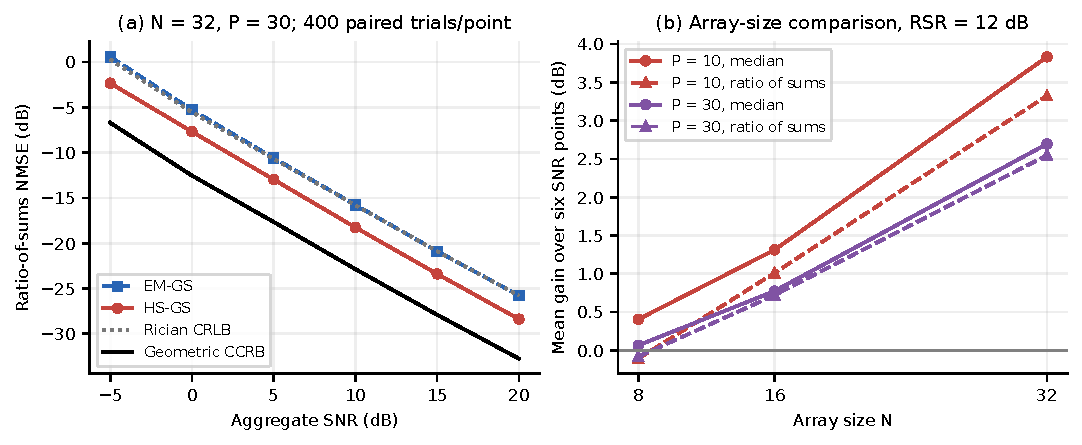
\includegraphics[width=\textwidth]{classical_array.pdf}
\caption{Classical study. Left: NMSE and information references at $N=32$, $P=30$, RSR 12~dB. Right: HS-amplitude gain versus array size for two pilot counts. HS-GS denotes four-sweep HS-amplitude. Solid gain curves average paired medians over six SNRs; dashed curves average ratio-of-sums gains.}
\label{fig:classical}
\end{figure*}
At $N=32$, $P=30$, RSR 12~dB, HS-amplitude gains 2.54--2.97~dB in paired median over EM-GS across six SNRs, averaging 2.70~dB (Fig.~\ref{fig:classical}). Ratio-of-sums gaps are 2.38--2.90~dB. At SNR at least 5~dB, EM-GS is within 0.108~dB of the Rician CRLB. The geometric CCRB is 6.95--7.06~dB below that reference, while HS-amplitude remains 4.37--4.85~dB above it. These local unbiasedness references do not establish efficiency or attainable headroom for the biased filtered estimates.

Averaging two pilot counts and six SNRs, paired-median gains are 0.236, 1.044 and 3.264~dB for $N=8,16,32$; ratio-of-sums gains are $-0.095$, 0.866 and 2.938~dB. Larger arrays provide more spatial samples of the same paths. At $N=8$, maximum Hankel rank is four and filtering is bypassed in 42.94\% of trials. A positive median alongside a negative total-error gain shows why aggregation matters.

\subsection{Effective Rank and Filtering Bias}
For the true noiseless Hankel spectrum, define effective rank~\cite{royvetterli2007}
\begin{equation}
 r_{\rm eff}=\exp(-\textstyle\sum_i p_i\log p_i),\qquad \rho=r_{\rm eff}/q.
\end{equation}
A spectrum dominated by a few values has low effective rank even if its algebraic rank is larger. We report median $\rho$ over users and worlds. This true-channel diagnostic is not available to the estimator.
\begin{figure}[!t]
\centering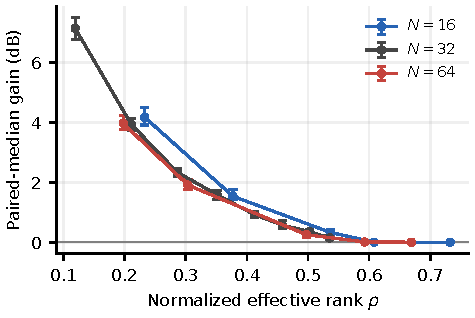
\includegraphics[width=\columnwidth]{effective_rank.pdf}
\caption{Four-sweep HS-amplitude paired-median gain versus true-channel normalized effective rank. Arrays use $P=20$, RSR 10~dB and the same random-SNR distribution. Bars are pointwise paired-bootstrap intervals. This is a diagnostic trend, not an observable switching threshold.}
\label{fig:rank}
\end{figure}
Across the matched array tests, hard-rank benefit generally falls as $\rho$ rises (Fig.~\ref{fig:rank}). At $N=32$, $\rho=0.536$ gives median gain 0.141~dB with interval $[0.090,0.211]$~dB. A value near one-half of capacity marks a small benefit here, not a universal threshold. At $N=16$, $L=14$, $\rho=0.732$, forcing rank seven loses 0.154~dB, with interval $[0.111,0.201]$~dB for the loss.

Adaptive rank does not protect every channel: at $N=32$, $L=14$, SNR 0~dB, HS-amplitude is worse than EM-GS in 47.75\% of 400 worlds. Selecting below the physical path count is not always harmful either. At $L=7$, SNR 0~dB, 78.75\% select below rank seven, but only 8.75\% of all worlds are worse than EM-GS.

Classical smooth filtering gains 0.914, 1.382 and 1.413~dB over four hard sweeps at SNR 0~dB for $L=3,7,14$. At 10~dB, gains are 0.005, 0.623 and 0.773~dB; the first interval includes zero. Learning is therefore not required to improve hard truncation. A separate historical check also finds one hard sweep better than four in all six cells by 0.275--0.652~dB. More filtering is not automatically better.


\subsection{What the Historical Learned Study Establishes}
An earlier, separately frozen 126-condition comparison used the original 21-context trained models, including path counts up to 16 and SNRs down to $-10$~dB. On its 4,032 primary worlds, the 188-parameter controller improved equal-cell NMSE by 1.835~dB over global filtering and 1.967~dB over a matched recurrent adaptation, with adjusted intervals $[1.805,1.871]$ and $[1.932,2.006]$~dB. A per-block rank-selected OptShrink adaptation was 0.452~dB more accurate on that study's main score and substantially slower. These observations support the adaptive component under that training/test design; they are not results for the final hybrid or its current operating grid. The full historical comparisons, including contrary rankings under pooled error and alternative training, remain in the supplement.

\subsection{Fresh Accuracy, BER and Runtime}
\begin{table*}[!t]
\centering
\caption{Fresh 153-condition comparison. Lower values are better. Runtime is the slower of two independently timed windows, in milliseconds.}
\label{tab:reliability-main}
\small
\setlength{\tabcolsep}{4pt}
\begin{tabular}{lrrrrr}
\toprule
Method & \shortstack{Mean-cell\\NMSE (dB)} & \shortstack{Pooled linear\\NMSE} & BER (\%) & \shortstack{Full-grid\\p90 (ms)} & \shortstack{Weak-target\\p90 (ms)} \\
\midrule
Reliability receiver & -38.620 & 0.00897384 & 0.522496 & 7.254 & 7.031 \\
Prior selective EM & -38.113 & 0.00900482 & 0.522496 & 7.148 & 6.809 \\
Full repaired receiver & -37.858 & 0.00903694 & 0.522571 & 14.690 & 14.858 \\
Adaptive start + EM40 & -35.691 & 0.02637969 & 0.808204 & 9.040 & 8.704 \\
Global schedule + EM40 & -36.482 & 0.02658368 & 0.813718 & 7.103 & 6.745 \\
Classical start + EM40 & -32.005 & 0.02744311 & 0.809387 & 7.142 & 6.802 \\
Spectral EM100 & -30.562 & 0.02839215 & 0.828828 & 8.835 & 8.752 \\
Compact sparse/EM & -31.895 & 0.00868525 & 0.489159 & 9.516 & 8.756 \\
Algebraic start + EM20 & -36.534 & 0.02788204 & 0.835676 & 3.101 & 2.747 \\
\bottomrule
\end{tabular}
\par\vspace{2pt}
\begin{minipage}{0.98\textwidth}\footnotesize Neural rows average metrics from three separately evaluated fits, not ensembles. Mean-cell NMSE equally averages condition-level dB ratios of summed error to summed channel energy; pooled linear NMSE first pools all conditions within each fit and then averages the fit ratios. The weak target is RSR 5~dB and SNR $>30$~dB (24 conditions). The declared runtime target is 10.74~ms in both scopes and both windows; it is not a per-call deadline. Compact sparse/EM includes zero-penalty EM choices and remains best in pooled-linear NMSE and aggregate BER.\end{minipage}
\end{table*}

Table~\ref{tab:reliability-main} is the final, fresh matched comparison. The new receiver improves equal-cell mean NMSE by 0.507~dB over the prior hybrid, with adjusted interval $[0.338,0.652]$~dB, and by 0.762~dB over the full repair, with interval $[0.231,0.878]$~dB. The prior-relative fit-specific gains are 0.497, 0.504 and 0.521~dB. Gains over the full repair vary more, at 0.361, 0.114 and 1.810~dB; averaging fits does not remove this dependence on the trained weights.

Observed aggregate BER is identical for the new and prior hybrids: 0.522496\%. The full repair has 17 additional errors across the three fits, all in one fit, but the adjusted interval for BER improvement includes zero. We therefore claim no established BER improvement over either primary comparator. Compact sparse/EM is better in aggregate BER (0.489159\%) and pooled linear NMSE (0.008685 versus 0.008974). It also has smaller pooled error-tail summaries. The new receiver's best equal-cell mean dB score does not imply dominance under every error aggregation or in communication reliability.

\begin{figure*}[!t]
\centering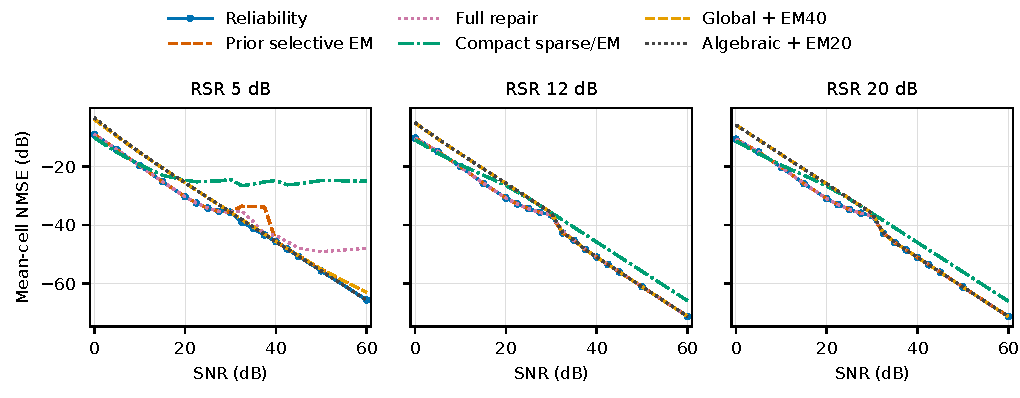
\includegraphics[width=\textwidth]{reliability_nmse.pdf}
\caption{Fresh final comparison. Each point averages the three path-regime cell NMSE scores; trained families additionally average three fit scores, not channel predictions. Curves are descriptive. All methods share observations. The algebraic-only and fixed-schedule controls show that classical recovery and a fixed trained schedule are strong at high SNR.}
\label{fig:reliability-nmse}
\end{figure*}
\begin{figure*}[!t]
\centering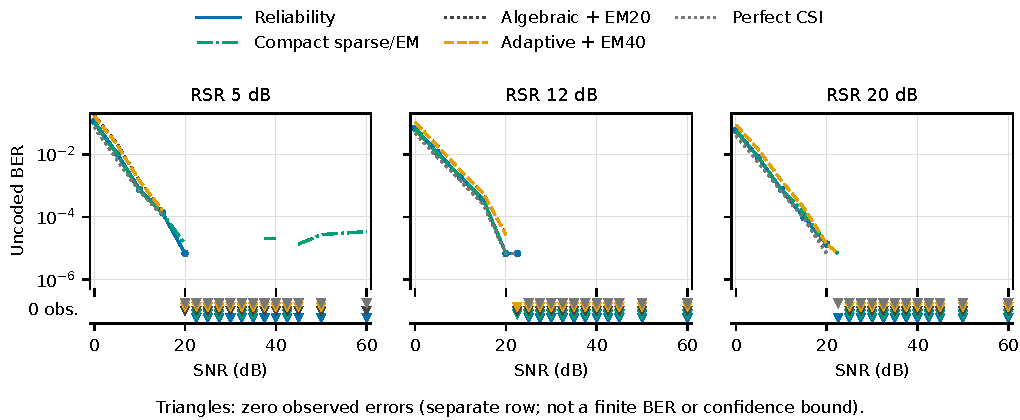
\includegraphics[width=\textwidth]{reliability_ber.pdf}
\caption{Estimate-then-detect BER on the same fresh observations and joint Rician detector. Points average path-regime rates, with equal case/bit counts. Zero-error observations appear in a separately labelled display row; they are not numerical upper bounds or evidence of equivalence. The perfect-CSI curve uses unavailable channel truth only as a detector diagnostic.}
\label{fig:reliability-ber}
\end{figure*}

\subsection{Where the New Check Helps and Where It Does Not}
\begin{table*}[!t]
\centering
\caption{Descriptive operating-range results on the same fresh bank.}
\label{tab:reliability-regions}
\small
\setlength{\tabcolsep}{4pt}
\begin{tabular}{llrrrrr}
\toprule
Region & Metric & Reliability & \shortstack{Prior selective\\EM} & Full repair & Sparse/EM & Algebraic20 \\
\midrule
Ordinary (45) & dB & -20.242 & -20.242 & -20.242 & -18.964 & -15.470 \\
 & BER (\%) & 1.776440 & 1.776440 & 1.776440 & 1.662191 & 2.841254 \\
Weak target (24) & dB & -48.644 & -45.411 & -43.893 & -25.607 & -48.457 \\
 & BER (\%) & 0.000000 & 0.000000 & 0.000480 & 0.001441 & 0.000000 \\
High SNR (45) & dB & -56.744 & -56.512 & -54.638 & -44.052 & -56.754 \\
 & BER (\%) & 0.000000 & 0.000000 & 0.000196 & 0.000633 & 0.000000 \\
\bottomrule
\end{tabular}
\par\vspace{2pt}
\begin{minipage}{0.98\textwidth}\footnotesize Ordinary: SNR $\leq20$~dB, all references. Weak target: RSR 5~dB and SNR $>30$~dB. High SNR: SNR $\geq40$~dB, all references. These scopes overlap and are not the multiplicity-adjusted primary comparisons. A displayed zero BER means no observed bit errors; it is neither a zero-error guarantee nor evidence of population equivalence. The first three methods are bitwise identical in the ordinary region.\end{minipage}
\end{table*}

The targeted region is reference 5~dB and SNR above 30~dB: 24 conditions. Here the receiver achieves $-48.644$~dB, improving on the prior by 3.232~dB, with descriptive interval $[2.249,3.966]$~dB, and on the full repair by 4.750~dB, with interval $[1.836,5.326]$~dB. Its pooled linear NMSE is $3.879\times10^{-5}$, versus $2.367\times10^{-4}$ for the prior. The fallback triggers on approximately 26.7--27.0\% of target cases across fits; every triggered fallback is accepted on this test bank and none has an invalid design. Trigger and acceptance remain separate decisions in the algorithm.

Fifteen of 153 condition-mean NMSE scores improve over the prior, with the remainder tied and none worse. This is a statement about the sampled condition means, not every individual channel. Ordinary-SNR outputs and all conditions outside the new gate are identical to the prior. Both methods have zero observed target-region bit errors, so the large channel-error gain has no measured BER benefit there.

The receiver does not beat the full repair in every cell: 32 condition means are worse, eight with pointwise intervals excluding zero. The largest mean loss is 0.701~dB at two paths, reference 20~dB and SNR 32.5~dB, outside the new gate. Under strong references at SNR at least 40~dB, its mean score is $-58.555$~dB versus $-58.558$~dB for the full repair. These residual losses are retained, rather than removed by test-dependent threshold changes.

Standalone algebraic-plus-EM20 is particularly competitive in the target region ($-48.457$~dB) and is the fastest tabulated pipeline. Its whole-grid BER, 0.835676\%, is substantially worse than the hybrid's. This supports combining components over the declared grid, while showing that learning is not necessary for accurate high-SNR recovery. The compact sparse/EM BER advantage is concentrated in ordinary-SNR operation, which this repair preserves rather than improves.

\subsection{Processing Budget and Latency Variability}
The new receiver passes both required p90 tests in both windows. Whole-grid p90 is 4.282 and 7.254~ms; target-region p90 is 4.162 and 7.031~ms. The fallback-triggered branch has p90 3.501 and 5.918~ms. Its conditional mix of operating points differs from that of untriggered calls, so these numbers do not imply that adding a fallback reduces cost. Every receiver reference/SNR-bin p90 also remains below 10.74~ms in the measured samples.

The slower second window affects the baselines as well. We retain both runs and report the worse p90; the full repair passes in the first window but fails in the second, at 14.690~ms overall and 14.858~ms in the target region. The final receiver has maximum measured times of 5.225 and 22.276~ms. One of its 1,377 calls in the second window exceeds 10.74~ms; its fallback gate was false. We do not assign a cause from these measurements. Thus the receiver meets the percentile target, not a hard per-call deadline.

\subsection{Negative Evidence and Scope}
The development record includes pilot-matched retraining, high-SNR bypass, weak-reference transition corrections, a filter-continuation repair around 40~dB, native-kernel runtime reduction and matched-start comparisons. These motivated the frozen final design. Earlier winners, failed confirmation tests and test-driven exploratory repairs are archived as development evidence, not independent confirmation of every component. No final-test outcome changes the selected rule.

Historical nearly noiseless tests exposed a large bias from nonvanishing learned filtering, even when initialized at the true channel. Historical variance and reference-phase perturbations also caused degradation. The final receiver has not been validated under those mismatches merely because its matched-model test is better. Known reference phase and variance remain required; constant reference-phase error can be absorbed by channel rotation and is not identified by a fitting-likelihood check. The current algebraic validity rule rejects constant-modulus fitting pilots. Array geometry, user counts other than three, hardware readout, nonlinear atomic dynamics and practical coded links require separate tests of the final pipeline.

\section{Discussion and Conclusion}
The learned controller and the reliability wrapper solve different problems. The controller reuses offline training to choose smooth structural corrections from spectral and residual features. The wrapper limits damage from some unfavorable solutions by trying a different classical initialization and checking its observable fitting loss. A useful complete receiver can contain both. Calling the accepted algebraic replacement a learned estimate, or claiming that more EM or stronger filtering is always helpful, would misattribute the results.

The analysis also separates distinct guarantees. Full-rank intensity regression gives exact noiseless recovery under its stated pilot/reference assumptions. The acceptance comparison ensures nonincrease of computed fitting loss relative to the prior. A smooth-filter norm bound constrains correction size. None implies global convergence, channel-error contraction, optimal shrinkage, arbitrary-pilot recovery or guaranteed BER improvement for the complete hybrid. The final empirical confirmation is conditional on calibrated observations and the declared populations.

An adaptive stage costs $O(NKP+NK^2+K^3+Kmq^2+Kq^3)$ in the dense implementation. The global schedule avoids adaptive feature/controller evaluation but still uses measurement updates and structural solves. With $d=K^2+2K$, the algebraic branch requires a real design solve of order $O(Pd^2+d^3+NPd)$, followed by its EM continuation; here $d=15$. Neural parameter count alone does not capture either online latency or offline data/calibration cost. The complete paired fit stores 218 neural parameters, plus policy entries, and uses extra held-out observations and known symbols during offline policy development.

On the fresh test, the new check improves the prior hybrid's equal-cell NMSE without an observed BER penalty and satisfies the 10.74~ms p90 target in both isolated timing windows. It improves high-SNR weak-reference recovery while preserving ordinary-SNR outputs. Compact sparse/EM retains better pooled linear NMSE and aggregate BER; standalone algebraic refinement is strong at high SNR. The paper's contribution is therefore a specified and reproducible combination of exact measurement updates, compact learned structure and observable classical recovery, with measured benefits and limits. It is not a claim that a learned estimator universally replaces classical estimation.

\subsection{Reproducibility and Remaining Comparisons}
The accompanying source package contains the final protocol, policy, numerical summaries, method/source/checkpoint hashes, verification records and figure/table inputs. Five final audits verify selection, channel estimates, BER, aggregate statistics and timing. Independent standalone and gate replays match the saved predictions exactly; the independent bootstrap reconstruction differs by at most $2.13\times10^{-14}$. The audits preserve the nine-block sampling dependence and all four adjusted primary outcomes. Historical evidence has its own protocol and sample counts; it is not pooled into the final comparison.

The manuscript source archive is self-contained for compilation, but is not a complete public release of all raw simulations and trained weights. A permanent code/data archive remains to be assigned. The three fits share a training dataset and the intervals condition on those fits. Full LRHD and published URformer remain unreproduced comparisons. Robustness to calibration error, constant-modulus-pilot redesign and independent training-population replications would strengthen the evidence; the present paper makes no claim that these have been completed.

\section*{Acknowledgment}
OpenAI's ChatGPT/Codex assisted with manuscript drafting and revision, experiment-code development, and figure-generation scripts. The author is responsible for verifying the content and final submission.
\bibliographystyle{IEEEtran}
\bibliography{references}
\end{document}
